Setelah informasi geometris dari LiDAR dan informasi termal dari kamera diperoleh, tahap berikutnya adalah mengintegrasikan kedua sumber data tersebut ke dalam representasi yang dapat digunakan oleh sistem navigasi. Integrasi dilakukan melalui dua mekanisme utama. Pertama, obstacle termal yang berada pada area \textit{blind-spot} LiDAR diproyeksikan menjadi \textit{Virtual LaserScan} sehingga dapat diproses oleh ROS Navigation Stack sebagaimana data LiDAR konvensional. Kedua, informasi traversability yang dihasilkan masing-masing sensor digabungkan untuk menghasilkan nilai traversability efektif yang digunakan sebagai masukan bagi pengendali fuzzy.

Pendekatan ini memungkinkan sistem memanfaatkan keunggulan masing-masing sensor secara komplementer. LiDAR menyediakan informasi geometris dengan akurasi tinggi, sedangkan kamera termal mampu mendeteksi obstacle yang tidak teramati oleh bidang pindai LiDAR (\cite{Choi2023,Schichler2025}).

\subsection{Pembentukan Virtual LaserScan dari Kamera Termal}
\label{sec:virtual_laserscan}

Informasi obstacle yang diperoleh dari topik \texttt{/thermal\_obstacle\_mask} tidak dapat digunakan secara langsung oleh ROS Navigation Stack karena masih berada dalam domain citra. Oleh karena itu, penelitian ini membentuk representasi \textit{Virtual LaserScan} yang memiliki format identik dengan keluaran sensor LiDAR.

Proses ini dilakukan oleh node \texttt{thermal\_blindspot\_to\_scan.py}. Node tersebut mene\-rima citra biner obstacle termal beresolusi $640 \times 480$ piksel dengan frekuensi 10 Hz, kemudian menghasilkan topik \texttt{/thermal\_blindspot\_scan} dalam format \texttt{sensor\_msgs/LaserScan}. Dengan pendekatan ini, obstacle termal dapat diproses oleh \textit{costmap} dan APFPlanner tanpa memerlukan modifikasi pada struktur ROS Navigation Stack.

Virtual scan dibentuk menggunakan 61 \textit{beam} yang tersebar pada rentang sudut

\begin{equation}
\theta \in [-0.70,\;0.70]\;\text{rad}
\end{equation}

atau sekitar $\pm 40^\circ$ terhadap arah depan robot. Rentang ini dipilih karena area tersebut merupakan zona yang paling relevan terhadap proses penghindaran obstacle pada navigasi lokal.

\subsection{Proyeksi Obstacle Blind-Spot ke Koordinat Robot}

Sebelum dilakukan proyeksi, masker obstacle termal terlebih dahulu diproses menggunakan operasi morfologi untuk mengurangi noise dan memperbaiki kontinuitas area obstacle. Operasi \textit{opening} digunakan untuk menghilangkan blob kecil yang tidak relevan, sedangkan \textit{closing} digunakan untuk menutup celah pada area obstacle.

Selanjutnya diterapkan pembatasan \textit{region of interest} (ROI) pada 55\% bagian bawah citra. Langkah ini dilakukan karena area tersebut merepresentasikan ruang yang berada dekat dengan robot dan paling berpotensi menyebabkan kolisi. Struktur panas yang berada jauh dari robot tidak dipertimbangkan pada tahap ini karena tidak berkontribusi langsung terhadap keputusan navigasi (\cite{Kibii2022}).

Setiap blob obstacle yang lolos proses seleksi kemudian diproyeksikan ke koordinat polar robot. Posisi vertikal piksel digunakan untuk mengestimasi jarak obstacle terhadap robot, sedangkan posisi horizontal digunakan untuk menentukan arah obstacle relatif terhadap sumbu depan robot.

Jarak estimasi dihitung menggunakan persamaan

\begin{equation}
r = r_{far} + (r_{near}-r_{far})v
\label{eq:range_projection}
\end{equation}

dengan

\begin{equation}
v=\frac{p_y-y_{top}}{h-y_{top}}
\end{equation}

di mana:

\begin{itemize}
\item $r$ adalah estimasi jarak obstacle,
\item $r_{near}$ adalah jarak minimum yang diasosiasikan dengan bagian bawah citra,
\item $r_{far}$ adalah jarak maksimum yang diasosiasikan dengan bagian atas ROI,
\item $p_y$ adalah koordinat vertikal piksel,
\item $h$ adalah tinggi citra.
\end{itemize}

Sementara itu, sudut obstacle dihitung menggunakan

\begin{equation}
u=\frac{p_x-w/2}{w/2}
\end{equation}

\begin{equation}
\theta=-u\alpha_{fov}
\label{eq:angle_projection}
\end{equation}

dengan:

\begin{itemize}
\item $p_x$ adalah koordinat horizontal piksel,
\item $w$ adalah lebar citra,
\item $\alpha_{fov}$ adalah setengah sudut pandang kamera termal.
\end{itemize}

Hasil proyeksi tersebut digunakan untuk mengisi nilai jarak pada \textit{beam} Virtual LaserScan. Dengan demikian, obstacle yang berada pada area blind-spot LiDAR dapat direpresentasikan sebagai obstacle virtual dalam sistem navigasi.

\begin{figure}[H]
\centering
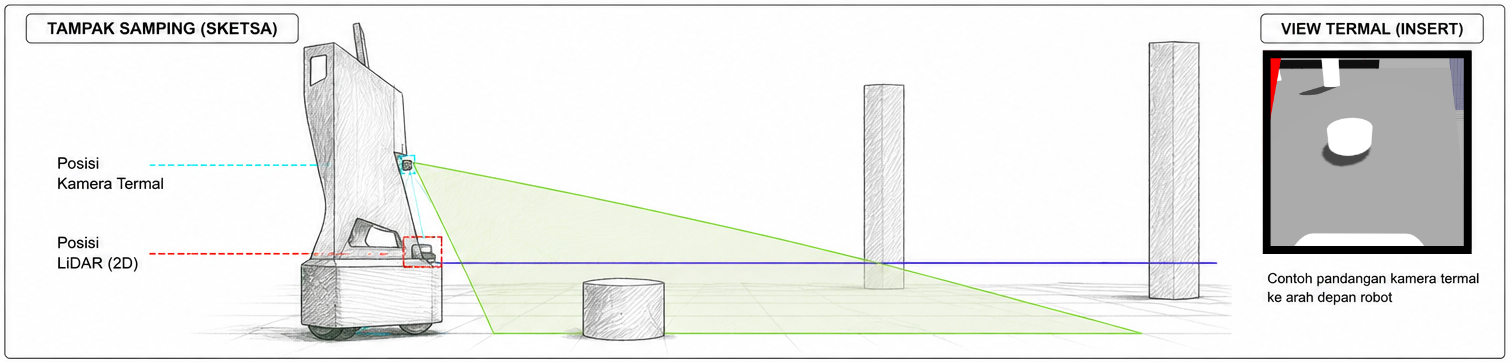
\includegraphics[width=0.85\textwidth]{gambar/3.6_proyeksi_blindspot.png}
\caption{Proses proyeksi obstacle termal ke koordinat polar robot untuk pembentukan Virtual LaserScan.}
\label{fig:proyeksi_blindspot}
\end{figure}

Untuk meningkatkan stabilitas deteksi, sistem menerapkan mekanisme memori temporal. Ketika obstacle termal menghilang sesaat akibat fluktuasi citra atau pergerakan kamera, hasil deteksi terakhir dipertahankan selama interval tertentu sebelum dihapus. Pendekatan ini mencegah terbentuknya perilaku navigasi yang tidak stabil akibat hilangnya obstacle secara tiba-tiba.

\subsection{Traversability Berbasis LiDAR}

Selain digunakan untuk mendeteksi obstacle, data LiDAR juga dimanfaatkan untuk meng\-estimasi tingkat keterlaluan lingkungan di sekitar robot. Konsep traversability digunakan untuk menggambarkan seberapa aman suatu area untuk dilalui berdasarkan ruang bebas yang tersedia (\cite{Sevastopoulos2022}).

Pada penelitian ini, traversability LiDAR dihitung berdasarkan lebar koridor bebas yang tersedia di sekitar arah pergerakan robot. Jarak lateral terhadap obstacle pada sisi kiri dan kanan diperoleh melalui proyeksi komponen jarak LiDAR terhadap sumbu lateral robot.

\begin{equation}
d_{lat}=r_i\sin|\varphi_i|
\label{eq:lateral_distance}
\end{equation}

dengan:

\begin{itemize}
\item $r_i$ adalah jarak LiDAR pada sudut $\varphi_i$,
\item $d_{lat}$ adalah komponen jarak lateral terhadap obstacle.
\end{itemize}

Lebar koridor bebas dihitung sebagai

\begin{equation}
w_{corridor}=d_{left}+d_{right}
\label{eq:corridor_width}
\end{equation}

Nilai tersebut kemudian dinormalisasi menjadi skor traversability LiDAR

\begin{equation}
\tau_{LiDAR}
=
\mathrm{clip}
\left(
\frac{w_{corridor}-w_{robot}}
{w_{ref}},
0,
1
\right)
\label{eq:trav_lidar}
\end{equation}

dengan:

\begin{itemize}
\item $w_{robot}$ adalah lebar robot,
\item $w_{ref}$ adalah lebar koridor referensi.
\end{itemize}

Semakin besar ruang bebas yang tersedia, semakin tinggi nilai traversability yang diperoleh.

\subsection{Fusi Traversability LiDAR--Termal}

Skor traversability yang dihasilkan LiDAR dan kamera termal memiliki karakteristik yang berbeda. Traversability LiDAR menggambarkan kondisi geometris lingkungan, sedangkan traversability termal merepresentasikan keberadaan obstacle berdasarkan informasi panas.

Sebelum dilakukan fusi, nilai traversability termal terlebih dahulu diproses menggunakan \textit{low-pass filter} asimetris. Filter ini dirancang agar sistem dapat merespons kemunculan obstacle secara cepat, namun tetap menghindari perubahan keputusan yang terlalu agresif ketika obstacle menghilang.

Koefisien filter didefinisikan sebagai

\begin{equation}
\alpha=
\begin{cases}
0.50, & \tau_{thermal}<\hat{\tau}_{thermal}\\
0.20, & \tau_{thermal}\geq\hat{\tau}_{thermal}
\end{cases}
\label{eq:lpf_alpha}
\end{equation}

dan pembaruan nilai traversability termal terfilter diberikan oleh

\begin{equation}
\hat{\tau}_{thermal}
=
(1-\alpha)\hat{\tau}_{thermal}
+
\alpha\tau_{thermal}
\label{eq:lpf_update}
\end{equation}

dengan:

\begin{itemize}
\item $\tau_{thermal}$ adalah traversability termal saat ini,
\item $\hat{\tau}_{thermal}$ adalah traversability termal hasil penyaringan.
\end{itemize}

Setelah proses penyaringan selesai, nilai traversability efektif dihitung menggunakan operator minimum

\begin{equation}
\tau_{eff}
=
\min
\left(
\tau_{LiDAR},
\hat{\tau}_{thermal}
\right)
\label{eq:trav_eff}
\end{equation}

Pendekatan ini menerapkan prinsip \textit{safety-first fusion}, yaitu sistem selalu menggunakan kondisi yang paling konservatif dari kedua sensor (\cite{Haider2022,Schichler2025}). Dengan demikian, apabila salah satu sensor mendeteksi kondisi yang tidak aman, nilai traversa\-bility efektif akan menurun sehingga robot dapat merespons lingkungan secara lebih hati-hati.

Nilai traversability efektif $\tau_{eff}$ bersama jarak obstacle terdekat $d_{obs}$ selanjutnya digunakan sebagai masukan pada pengendali fuzzy Mamdani yang akan dijelaskan pada subbab berikutnya.